

\documentclass[tikz]{standalone}
\usepackage{tikz}
\usepackage{pgfplots}
\usepackage{tikz-layers}
\usepackage{amsmath}
\usepackage{bm}

\newcommand{\X}{\mathbf{X}}
\newcommand{\w}{\mathbf{w}}
\newcommand{\x}{\mathbf{x}}
\newcommand{\uu}{\mathbf{u}}
\newcommand{\h}{\mathbf{h}}
\newcommand{\y}{\mathbf{y}}
\newcommand{\dist}{\mathbf{d}}
\newcommand{\Y}{\mathbf{Y}}
\newcommand{\g}{\mathbf{g}}
\newcommand{\e}{\mathbf{e}}
\newcommand{\U}{\mathbf{U}}
\newcommand{\res}{\mathbf{r}}
\newcommand{\regr}{\bm{\varphi}}
\newcommand{\hest}{\hat{\mathbf{h}}}
\newcommand{\yest}{\hat{\mathbf{y}}}
\newcommand{\norm}[1]{\Vert {#1} \Vert_2}
\newcommand{\normone}[1]{\Vert {#1} \Vert_1}
\newcommand{\norms}[1]{\Vert {#1} \Vert_2^2}
\newcommand{\conj}[1]{{#1}^*}
\newcommand{\vars}{\hat{\sigma}_e^2}
\newcommand{\var}[1]{\mathrm{Var[{#1}]}}
\newcommand{\E}[1]{\mathrm{E[{#1}]}}
\newcommand{\BigO}[1]{\ensuremath{\operatorname{O}\bigl(#1\bigr)}}

\definecolor{mycolor1}{RGB}{0,98,155}%
\definecolor{mycolor2}{RGB}{186 12 47}%
\definecolor{mycolor3}{RGB}{255 163 0}%
\definecolor{mycolor4}{RGB}{255 209 0}%
\definecolor{mycolor5}{RGB}{120 190 32}%
\definecolor{mycolor6}{RGB}{0 132 61}%
\definecolor{mycolor7}{RGB}{152 29 151}%
\definecolor{mycolor8}{RGB}{0 156 166}
\definecolor{mycolor9}{RGB}{0 181 226}
\definecolor{mycolor10}{RGB}{134 31 65}
\definecolor{mycolor11}{RGB}{232 119 34}
\definecolor{mycolor12}{RGB}{255 199 34}
\definecolor{mycolor13}{RGB}{101 141 27}
\definecolor{mycolor14}{RGB}{0 99 65}
\definecolor{mycolor15}{RGB}{119 37 131}
\definecolor{mycolor16}{RGB}{0 115 119}
\definecolor{mycolor17}{RGB}{0 40 85}
\definecolor{forward}{RGB}{235 23 0}%
\definecolor{feedback}{RGB}{31, 7, 217}%

\usetikzlibrary{shapes,arrows,fit,backgrounds,calc}
\usetikzlibrary{automata,positioning}

\tikzstyle{block} = [draw, fill=blue!20, rectangle,
    minimum height=3em, minimum width=6em]
\tikzstyle{sum} = [draw, fill=blue!20, circle, node distance=1cm]
\tikzstyle{input} = [coordinate]
\tikzstyle{output} = [coordinate]
\tikzstyle{pinstyle} = [pin edge={to-,thin,black}]


\tikzset{%
    gain/.style     = {draw, thick, isosceles triangle, minimum height = 3em,
        isosceles triangle apex angle=60},
    block/.style    = {draw, thick, rectangle, minimum height = 3em,
        minimum width = 3em, fill=white},
}

\tikzset{
    schritt/.style={
        draw,
        rounded corners,
        fill=blue!20,
        inner xsep=2em,
    },
    background/.style={
        draw,
        fill=yellow!30,
        align=right
    }
}

\pgfdeclarelayer{bg}    % declare background layer
\pgfsetlayers{bg,main}  % set the order of the layers (main is the standard layer)

\newcommand{\extendnode}[1]{
    (#1)
    ($(current bounding box.north east)!(#1)!(current bounding box.south east)$)
    ($(current bounding box.north west)!(#1)!(current bounding box.south west)$)
}
\begin{document}
% The block diagram code is probably more verbose than necessary

% \begin{tikzpicture}[auto, node distance=2cm,>=triangle 45]
%     % We start by placing the blocks
% %    \node [input, name=input] {};
% %    \node [input, below of = input, name=input2] {};

%     \node [block, ,text width=2.5cm, node distance=4cm, align=center] (dpd) {$\mathbf{x}_1 = \mathbf{u}_1 - \mathbf{U}_1\mathbf{w}_1$\\$\mathbf{x}_2 = \mathbf{u}_2 - \mathbf{U}_2\mathbf{w}_2$};
%     \node[input, left=of dpd.150, name=input] {};
%     \node[input, left=of dpd.210, name=input2] {};


%     \node [block, right of=dpd,text width=1.5cm, node distance=5cm, align=center] (comb) {Synthesis Stage};
%     %\node [block, right of=comb,text width=1cm, node distance=2.5cm, align=center] (digtorf) {Digital to RF};
%     \node [gain, right of=comb, node distance=2cm, fill=white] (pa) {PA};
%     % We draw an edge between the digtorf and system block to
%     % calculate the coordinate u. We need it to place the measurement block.

%     \node [output, right of=pa] (output) {};

%     \node [block, below of=comb,text width=1.5cm, align=center] (sep) {Analysis Stage};
%     %\node [block, below of=digtorf,text width=1cm, align=center] (rftodig) {RF to Digital};

%     \node [block, below of=dpd, text width=2cm, align=center] (coeffsel) {$\mathbf{x}_1 = \mathbf{u}_1 - \mathbf{U}_1\mathbf{w}_1$};
%     \node [block, below of=coeffsel, text width=2cm, align=center] (ridge) {Ridge};

%     % Once the nodes are placed, connecting them is easy.
%     \draw [draw,->] (input) -- node {$\mathbf{u_1}$} (dpd.150);
%     \draw [draw,->] (input2) -- node {$\mathbf{u_2}$} (dpd.210);

%     \draw [->] ([yshift=+.3cm]dpd.east) -- node[name=dpdtodig] {$\mathbf{x_1}$} ([yshift=+.3cm]comb.west);
%     \draw [->] ([yshift=-.3cm]dpd.east) -- node[name=dpdtodig] {$\mathbf{x_2}$} ([yshift=-.3cm]comb.west);

%     \draw [->] (comb) -- node[name=u] {$\mathbf{u}$} (pa);

%     %\draw [->] (digtorf) -- node[name=u] {$\mathbf{u}_{\text{RF}}$} (pa);

%     \draw [->] (pa) -- node [name=y] {$\mathbf{y}$}(output);
%     \draw [->] ([yshift=-.1cm]y.south) |- (sep);
%     \draw [-] ([xshift=-.3cm,yshift=-.1cm]y.south) -- ([xshift=0cm,yshift=-.1cm]y.south);
%     % \draw [->] (rftodig) -| node[pos=0.99] {$-$}        node [near end] {$y_m$} (dpd);

%   %  \draw [->] (pa) -- node [label=$\mathbf{y}$] {}(sep);

%      \node [input, name=dpdcontroller1, above right = .4cm and .3cm of dpd] {};
%     \node [input, name=dpdcontroller2, below left = .2cm and .1cm of dpd] {};

%     \draw [->] ([yshift=+.3cm]sep.west) -- node[label=$\mathbf{y_1}$] {}([yshift=+.3cm]coeffsel.east);
%     \draw [->] ([yshift=-.3cm]sep.west) -- node[label=$\mathbf{y_2}$] {}([yshift=-.3cm]coeffsel.east);

%     \draw [-] ([xshift=0cm,yshift=-.1cm]input.south) -- ([xshift=.4cm,yshift=-.1cm]input.south);
%     \draw [-] ([xshift=0cm,yshift=-.1cm]input2.south) -- ([xshift=.3cm,yshift=-.1cm]input2.south);
%     \draw [->] ([xshift=.4cm,yshift=-.1cm]input.south) |- node {}([yshift=.3cm]coeffsel.west);
%     \draw [->] ([xshift=.3cm,yshift=-.1cm]input2.south) |- node {}([yshift=-.3cm]coeffsel.west);

% %    \draw [-] ([xshift=0cm,yshift=-.1cm]dpdtodig.south) -- ([xshift=.3cm,yshift=-.1cm]dpdtodig.south);

%     \draw [-,dashed] ([xshift=-.75cm]coeffsel.north) -- node {}(dpdcontroller2);
%         \begin{pgfonlayer}{bg}    % select the background layer
%         %\node [draw, thick, green!50!black, fill=green!75!black!25, rounded corners, fit=(dpd)(coeffsel), inner xsep=15pt, inner ysep=10pt] {};
%         %\node [draw, thick, blue!50!black, fill=blue!75!black!25, rounded corners, fit=(pa)(comb)(sep), inner xsep=15pt, inner ysep=10pt] {};


%         \fill [blue!50!black, fill=blue!75!black!25, rounded corners, fit=(pa)(comb)(sep), inner xsep=15pt, inner ysep=10pt] ([xshift=0.1cm,yshift=-0.5cm]sep.south) rectangle ([xshift=1.6cm,yshift=1cm]pa.center);
%         \fill [green!50!black, fill=green!75!black!25, rounded corners, fit=(dpd)(coeffsel), inner xsep=15pt, inner ysep=10pt] ([xshift=-2cm,yshift=1cm]dpd.center) rectangle ([xshift=-0.1cm,yshift=-0.5cm]sep.south);
%         \node[] at ([xshift=3.3cm,yshift=.2cm]comb.north)[text=blue!65!black] {$f_{sa}$};
%         \node[] at ([xshift=-0.5cm,yshift=.2cm]comb.north)[text=green!65!black] {$f_{int}$};


%         %\draw [draw, thick, green!50!black, fill=green!75!black!25, rounded corners, fit=(dpd)(coeffsel), inner xsep=15pt, inner ysep=10pt] ([xshift=-2cm,yshift=1cm]dpd.center) rectangle ([xshift=-0.1cm,yshift=-0.5cm]sep.south);
%         %\draw [draw, thick, blue!50!black, fill=blue!75!black!25, rounded corners, fit=(pa)(comb)(sep), inner xsep=15pt, inner ysep=10pt] ([xshift=0.1cm,yshift=-0.5cm]sep.south) rectangle ([xshift=1.6cm,yshift=1cm]pa.center);

%     \draw [->,densely dashdotted] (dpdcontroller2) -- node {}(dpdcontroller1);
%     \end{pgfonlayer}



% \begin{pgfonlayer}{bg}


%   %\path [use as bounding box] (current bounding box.north west) (current bounding box.south east); % Freeze current bounding box
%   %\node [fit={\extendnode{pa}}, background] {First};

% \end{pgfonlayer}

% \end{tikzpicture} 

\pgfdeclarelayer{bg}    % declare background layer
\pgfsetlayers{bg,main}  % set the order of the layers (main is the standard layer)

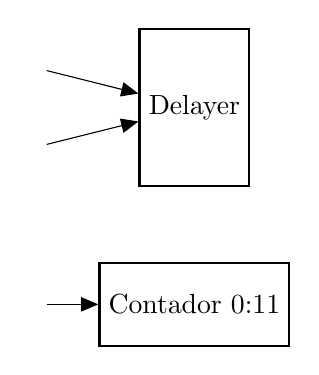
\begin{tikzpicture}[auto, node distance=2cm,>=triangle 45]
    % We start by placing the blocks
    \node [] (in_valid) {};
    \node [above of = in_valid] (in_imag) {};
    \node [above of = in_imag , yshift = -1cm] (in_real) {};
    

    \node [align =  center,block, right of = in_real, minimum height = 2cm, yshift = -0.5cm] (biest) {Delayer};
    \node [align = center,block, right of = in_valid](contador){Contador 0:11};
    \node [align =  center,block, right of = in_real, minimum height = 2cm, yshift = -0.5cm] (biest) {Delayer};
    \node [align = center,block, right of = in_valid](contador){Contador 0:11};
    
    
    
    %\node [input, left=of dpd, node distance=8cm, name=input] {};
    % \node [align=center,block,minimum height=5cm,xshift = 2cm,text width=2.5cm, right of = bits] (cSP) {Conversión Serie-Paralelo};

    % \node [align=center,block,minimum height=5cm,xshift = 2cm,xshift = 1cm,text width=3cm, right of = cSP] (mod) {Modulación Elegida QAM o PSK};

    % \node [align=center,block,minimum height=5cm,xshift = 2cm,xshift = 1cm,text width=2cm, right of = mod] (ifft) {IFFT};
    
    % \node [align=center,block,xshift = 1cm,text width=1.75cm, right of = ifft] (cp) {Inserción de CP};
    % \node [align = center,block,xshift = 1cm,minimum height=1.5cm,text width=2cm, right of = cp] (pulse) {Pulso Conformador};

    % % Once the nodes are placed, connecting them is easy.
    % \draw [draw,->] (bits) -- node {} (cSP);
    % \draw [draw,->,yshift = 1.65cm ] (cSP) -- node {} (mod);
    % \draw [draw,->,yshift = 1.1cm] (cSP) -- node {} (mod);
    % \draw [draw,->,yshift = 0.55cm] (cSP) -- node {} (mod);
    % \foreach \k in {-3,-2,-1,0,1,2,3}{
    %     \draw [->,line width = .25mm] ([yshift=\k*0.75cm]cSP.east) -- ([yshift=\k*0.75cm]mod.west);
    %  }
    % \foreach \k in {-3,-2,-1,0,1,2,3}{
    %     \draw [->,line width = .25mm] ([yshift=\k*0.75cm]mod.east) -- ([yshift=\k*0.75cm]ifft.west);
    % }
    % \draw [draw,->] (mod) -- node {} (ifft);
    % \draw [draw,->] (ifft) -- node {} (cp);
    % \draw [draw,->] (cp) -- node {} (pulse);
    %\draw [draw,->] (sep) -- node {} (suma);

    \draw [draw, ->] (in_real) -- node {} ([yshift = 0.5cm]biest);
    \draw [draw, ->] (in_imag) -- node {} ([yshift = -0.5cm]biest);
    \draw [draw, ->] (in_valid) -- node {} (contador);


\end{tikzpicture}
\end{document}